%%%%%%%%%%%%%%%%%%%%%%%%%%%%%% -*- Mode: Latex -*- %%%%%%%%%%%%%%%%%%%%%%%%%%%%
%% nsf.tex         : 2009 Smart Consumer Proposal
%% Author          : Philip Johnson
%% Created On      : Tue Mar 31 11:16:58 2009
%% Last Modified By: Philip Johnson
%% Last Modified On: Mon Oct 18 13:58:19 2010
%%%%%%%%%%%%%%%%%%%%%%%%%%%%%%%%%%%%%%%%%%%%%%%%%%%%%%%%%%%%%%%%%%%%%%%%%%%%%%%
%%   Copyright (C) 2009 
%%%%%%%%%%%%%%%%%%%%%%%%%%%%%%%%%%%%%%%%%%%%%%%%%%%%%%%%%%%%%%%%%%%%%%%%%%%%%%%
%% 
 
\documentclass[11pt]{article}
\usepackage[final]{graphicx}

\usepackage[nottoc,numbib]{tocbibind}

%% Make subsubsections numbered and included in ToC
\setcounter{secnumdepth}{3}
\setcounter{tocdepth}{3}

\usepackage{multirow}

%% URLs
\usepackage{url}
\usepackage[colorlinks, bookmarks=true]{hyperref}

%% Define a new 'smallurl' style for the package that will use a smaller font.
\makeatletter
\def\url@smallurlstyle{%
  \@ifundefined{selectfont}{\def\UrlFont{\sf}}{\def\UrlFont{\small\ttfamily}}}
\makeatother
%% Now actually use the newly defined style.
\urlstyle{smallurl}

%% CO2 
\usepackage{xspace}
\newcommand{\COtwo}{CO\ensuremath{_2}\xspace}

%% Make margins less ridiculous
\usepackage{fullpage}

%% Since I'm using the LaTeX Makefile that uses dvips, I need this
%% package to make URLs break nicely
\usepackage{breakurl}

\begin{document}
\title{The Kukui Cup: \\Proposal for a UH Residence Hall Energy Competition}

\author{Philip M. Johnson \\
Collaborative Software Development Laboratory \\
Department of Information and Computer Sciences \\
University of Hawai'i \\
johnson@hawaii.edu \\
\url{http://csdl.ics.hawaii.edu/techreports/10-03/10-03.pdf}
}

\maketitle

\tableofcontents
\newpage

\section{Executive Summary}

Kukui nut oil was used by ancient Hawaiians to light their homes.  In honor
of this original form of ``electricity'' in the islands, we propose to design and
implement a Residence Hall Energy Competition for the University of Hawaii called the
``Kukui Cup''.   It will be held for the first time during the month of October,
2011.  The three goals of this project are: (1) Improve the energy literacy
of participating students; (2) Conduct innovative research in information
technology for energy-related behavioral change; and (3) Save money for the
university by reducing energy costs.  As part of this project, we will
implement a new web application to provide information regarding UH Residence Hall
energy consumption in general and the Kukui Cup competition in particular.  This
software will also support research on energy behavior by the Collaborative
Software Development Laboratory in the Department of Information and
Computer Sciences.  We propose to hold the October, 2011 dorm energy
competition in three freshman dorms, and then expand the program to include
addition dorms in future years.

We propose the installation of Ethernet-connected energy meters into the
selected dorms that will provide sub-minute energy consumption data
regarding each ``lounge''\footnote{The Hale Aloha residence halls are
  configured such that electrical services are provided to pairs of floors
  (lounges) at a time.}.  We have developed a set of meter requirements for
this project including: the total number of meters, max current, required
energy data, data sampling interval, network communication, software
interface, internal storage, and submetering.  Our research indicates that
the Electro Industries Shark 200S is best suited to our requirements. 
We will develop software that will query each
meter via Ethernet at sub-minute intervals for current energy data and send
that information to a WattDepot energy data repository service for
collection and analysis.  The Residence Hall Energy web application will
then query the WattDepot service for energy data and analyses as required.

The Kukui Cup competition implements a variety of novel
features intended to support sustained, positive, behavioral change in
energy behaviors.  These features include: personalized, private pages;
near-real time display of energy consumption data; and a ``Kukui Nuts''
competition that implements a point system for actions intended to improve
energy literacy.  The competition provides incentives for three kinds of
actions: activities, goals, and commitments.  The design of the competition
is based upon prior research in behavioral change and will support data
collection and analysis to provide new insights into effective incentives
for energy conservation and information technology support.

The project involves a variety of stakeholders, including: the
Collaborative Software Development Laboratory, UH residence hall residents, UH 
residence hall advisors, UH Housing Office, UH Facilities, Sustainable UH, and
local energy organizations.  The needs of each of these stakeholders must
be identified and satisfied for this project to move forward.

The estimated budget for the first year of this project is \$60,945, based
upon: purchase of 31 meters and associated equipment (\$39,435);
installation of the meters (\$15,364); and funding for parties and prizes
(\$6,145).  The estimated direct return on this investment for the first
year of this project is approximately \$60,000, based upon a sustained 5\%
reduction in energy usage.  Because the purchase and installation of meters
is a one-time cost, we believe the project could begin saving the
University on the order of \$40,000 or more per year beginning in year
2012.


\newpage
\section{Goals}

This project has three primary goals:
\begin{enumerate}
\item Improve the {\em energy literacy} of the participating students;
\item Conduct {\em innovative research} in information technology for
  energy-related behavioral change;
\item {\em Save money} for the university by reducing energy costs.
\end{enumerate}

\subsection{Improve energy literacy}

Energy literacy \cite{DeWaters09b, DeWaters09} has three components:
knowledge, attitudes, and behaviors. Energy knowledge refers to factual 
information and skills, such as the ability to estimate the energy savings
in watt-hours from switching lights from incandescent to compact
fluorescent.   Energy attitudes refers to one's opinions and beliefs
related to energy, such as that conserving energy is good for
the environment.   Energy behaviors combine knowledge and attitudes to
produce concrete action, such as replacing the incandescent bulbs in one's
home with compact fluorescent. 

While one might assume from the above definition that energy literate
behaviors follow naturally from knowledge and attitudes, there is
substantial research to the contrary.  For example, Geller \cite{Geller81}
performed an experiment in which 40 consumers attended a three hour
workshop on energy conservation.  A pre and post workshop questionnaire
determined that all participants gained greater awareness of energy issues,
more appreciation for what could be done in their homes to reduce energy
use and save money, and a willingness to implement the changes that were
advocated in the workshop. However, a one month followup indicated very
little actual change in behavior. One person lowered the temperature on the
hot water heater. Two additional people had installed insulating blankets
around their hot water heaters, but they had already done this before the
workshop. Finally, eight people installed low-flow shower heads---after all
40 participants had been given the low-flow shower heads at the workshop.

As this and similar research illustrates, simply providing people with
information about energy, even if it affects their attitudes, is generally
not enough to create sustained, positive behavioral change with respect to
their energy usage.  Fortunately, there is also a growing body of research
on techniques that do support behavioral change
\cite{Becker78,Darby06,Faruqui09,Houwelingen89,Peterson07,Peterson07a,Staats04,Vollink99},
which can be summarized as follows.  First, provide {\em personalized
  information} that reflects the consumer's unique circumstances.  For
example, a dorm resident will not respond well to energy tips involving
improved insulation.  Second, provide both {\em general and specific
  commitments}, especially when they can be tied to a broader issue. For
example, pledging to use a clothesline rather than a dryer because it
reduces green house gas emissions.  Third, provide {\em achievable goals}
that can be objectively measured.  An example might be to reduce energy
consumption by 10\% over the previous month.  Fourth, elicit {\em social
  reinforcement} which can be manifested in both overt and subtle ways.
For example, in dorm settings, as more and more residents publicly
participate, it implicitly becomes ``the thing to do''.  Fifth, provide
{\em constant and contextual feedback} which helps verify progress toward
goals and can reinvigorate commitments, as long as the feedback is provided
in the right way at the right time.  Sixth, {\em financial incentives} can
be a powerful motivator for energy conservation. For example, a prize such
as iPods to the members of the dorm floor who conserved the most energy.

Thus, the first design goal of this project is to increase factual
knowledge about energy by participants, foster more sophisticated attitudes
based upon this knowledge, and, most finally, facilitate actual behavioral
change.  If we are successful in improving the energy literacy of
participants, their changes in behavior will be sustained beyond the
competition, and even beyond their time in the dormitories. 


\subsection{Conduct innovative IT energy research}

As noted in the previous section, there is evidence in support of a variety
of techniques for promoting sustained, positive behavioral change, but
current dorm energy competitions either do not employ these techniques, or
they do not utilize information technology effectively to deploy the
techniques or support assessment of their effectiveness.

The most common form of information technology support for dorm energy
competitions is a simple relatively static web site, as illustrated in
Figure \ref{fig:wellesley}.  These websites provide access to resources
about energy, and feedback regarding energy usage for the entire building
every few days.  The most sophisticated technology to date is the Campus
Resource Monitoring System at Oberlin College, which has the potential to
provide near-real time energy consumption data\footnote{With respect to
  energy consumption data, we define ``near-real time'' as sub-minute
  update intervals.  For example, obtaining meter data every 10 seconds is
  ``near real time'', while obtaining meter data every 15 minutes is not.}.

\begin{figure*}[!ht]
  \center
  \includegraphics[width=0.8\textwidth]{wellesley.ppt.eps}
  \caption{\em \small The Wellesley College Dorm Energy Competition Web site.}
 \label{fig:wellesley}
\end{figure*} 


We are designing a collection of software services that will provide UH
dorm residents participating in the competition with unparalleled
information technology support for improving their energy literacy.  Our
software will support a unique combination of features including: (a)
near-real time energy consumption data, (b) floor-level as well as
building-level energy data; (c) personalized, login-protected pages for
each student; (d) energy literacy activities with a ``Kukui Nut'' award
system for participation; and (e) integration with other information
technologies used by students, including text messaging, Facebook, email,
and Twitter.

Our software services are not designed merely to be cool or trendy; they
are designed to enable substantial, important research into energy
behavior. While prior research has generated evidence regarding a variety
of techniques for fostering behavioral change, there is relatively little
understanding of the relative importance or impact of these methods.  Our
software will enable us to present students with a variety of avenues for
participation and incentives and then track many of the ways in which they
participated. It will enable us to observe and record participant energy
usage (on a floor-by-floor basis) before, during, and after the
competition.  In addition, we will request student volunteers for an energy
literacy assessment both before and after the competition.  The result of
these three streams of data will provide a uniquely rich source of insight
into the popularity of various activities, their impact on energy literacy,
and the final impact on actual energy usage.

More details on the software are provided in Sections
\ref{sec:userinterface} and \ref{sec:features}, but in summary, the goal of
our software is to provide innovative support for improving energy literacy
in students combined with infrastructure to enable ground-breaking
empirical research in sustainability and energy.

\subsection{Save money}

The final goal is to save money.  Previous dorm energy challenges at
Brandeis University, Carleton College, Harvard University, MIT, Mount
Holyoke College, Ohio University, and Williams College have reported energy
savings, generally in the range of 7\% to 16\%.  If we can achieve these
results, and if the savings can be sustained for the remainder of the
school year, then energy costs for the dorms alone could be reduced by tens
of thousands of dollars\footnote{Section \ref{sec:budget} provides a more
  detailed analysis of the estimated costs and savings associated with this
  project}.

However, those are just the ``first-order'' savings to the university.  If
the competition achieves the goal of improving the energy literacy of
students, then their energy literate behavior will be manifested everywhere
on campus, not just in their dorm floors.  A more energy literate student
will choose energy saving behaviors in campus cafeterias, classrooms, and
labs, producing additional, ``second-order'' savings to the university.
Furthermore, the ``return on investment'' in improved energy literacy will
occur over their entire time at the university, not just during the one
month competition, and not just during their one year in the dorm.  We also
hope that these energy literate students will influence their friends in
positive ways, reaping additional dividends.

There is even the possibility of ``third-order'' savings.  We are designing
this project to begin with dormitory energy competitions, then extend into
residential community energy challenges \cite{csdl2-09-15}.  In addition,
we are releasing all software developed under this project as open source
in order to facilitate more wide-spread adoption.  Thus, this project could
lead to eventual energy cost savings in our community and elsewhere.

\section{Approach}
\label{sec:approach}

Our pursuit of the three goals of energy literacy, innovative research, and
saving money results in the following proposed approach to a UH Residence Hall
Energy competition.  

To summarize, we propose to hold the first annual Kukui Cup competition
during Fall semester of 2011.  The competition will involve all three of 
the Hale Aloha residence halls: Lehua, Ilima, and Mokihana.

During winter break of 2010, we will install meters in one of the freshman dorms. 
During Spring, 2011 semester, we will monitor energy usage in this dorm, conduct
focus groups, and evaluate our technologies. During summer, 2011, we will install
energy meters in the remainder of the dorms. 

The competition will be held during October, 2011.  We will continue to
monitor energy usage for the remainder of the year and conduct follow-up
studies to assess the impact and permanence of any energy reductions
observed during the competition period.

We plan to build upon the results from the first year to hold improved
versions in following years, hopefully expanding the number of involved
dorms as well. 

\subsection{User Interface}
\label{sec:userinterface}

\begin{figure*}[!ht]
  \center
  \includegraphics[width=1.0\textwidth]{home.2.png.eps}
  \caption{\em \small Home page mockup.}
 \label{fig:homepage}
\end{figure*} 

The public home page provides general information about energy usage, and
tabs to other pages including: a Resource page with links to further
information about energy usage and conservation; an Energy Data page that
displays charts generated from meter data; a Kukui Cup page that will
present current standings and activities related to the competition during
October, and more general information about it at other times of the year;
and an About page that provides contact information.

A distinguishing feature of our approach is a personalized private page that each
resident of the dorm can access by logging in to the site using their UH
account information.  Figure \ref{fig:mailepage} illustrates what such a
private page might provide for a hypothetical dorm resident named Maile Kalama.  In
addition to profile information, the page displays Maile's activities,
commitments, and goals, the current and cumulative energy usage of her
floor, and her individual and floor-level standings for the previous and
current rounds of competition.

\begin{figure*}[!ht]
  \center
  \includegraphics[width=1.0\textwidth]{maile.2.png.eps}
  \caption{\em \small Personalized page with individual and floor status.}
 \label{fig:mailepage}
\end{figure*} 

For more details on the site and its functionality, see Section \ref{sec:features}.

\subsection{Architecture}

The primary hardware and software components are summarized in Figure \ref{fig:architecture}.

\begin{figure*}[!ht]
  \center
  \includegraphics[width=1.0\textwidth]{architecture.ppt.eps}
  \caption{\em \small Basic architecture of the dorm energy data collection system.}
 \label{fig:architecture}
\end{figure*} 

Two Shark 200S energy meters will be installed on each Lounge of each dorm involved in
the competition. 

Each meter will have an Ethernet connection, and energy data from each
meter will be sent at sub-minute intervals to our software service,
WattDepot \cite{WattDepot}.  We directly connect each meter to the UH network via Ethernet,
rather than use a building-wide ModBus with a single Ethernet gateway, in
order to avoid bus contention that might occur due to the sub-minute
polling requirements for our system.

The energy data collected from each floor of each dorm at sub-minute
intervals is stored in WattDepot, which can perform various analyses
including aggregation and interpolation to transform it into a
convenient form for display within the web application.

We recognize that several aspects of our proposed architecture are unusual:
installing meters on every lounge (versus one for the entire building);
directly connecting each meter to Ethernet (versus using ModBus or a mesh
network); and sub-minute polling (versus 15 minute or greater polling).
These decisions are based upon our research into effective incentives for
sustained, positive behavioral change, which includes personalized,
constant, and contextual feedback.  

As a simple example, let's say that the residents of a dorm floor want to
figure out their ``baseline'' energy usage: how much electricity is used on
their floor after they turn off everything under their control.  If the
only meter available is at the building-level, the residents could not
succeed, since energy fluctuations in the remainder of the building would
drown out their action.  Similarly, if energy data from the meters is collected
only once every 15 minutes, the experiment becomes difficult to perform,
since they would have to keep everything off for an extended period of
time.  

Other behavioral incentives affected by this architecture include
personalized information and social norms.  By providing floor-level
meters, we can support competition between floors as well as between dorms.
This finer granularity of competition makes the actions of any individual
vastly more significant, since they are one of 24 members, as opposed to
one of 200 or more.

\subsection{Meters}
\label{sec:meters}

This proposal requires the installation of energy meters on each floor of
the dorms participating in the competition.  We conducted a review of
commercial building meters to determine which ones might be
suitable.  To support this process, we developed the list of
requirements summarized in Figure \ref{fig:meterrequirements} below:

\begin{figure}[!ht]
\small
\begin{tabular}{p{1.75in}p{4.25in}} \hline
{\bf Requirement} & {\bf Description}  \\
Total meters & 24 (estimate based on 2 dorms with 12 floors each) \\ 

Building power (BP) & 3 phase \\  

Max current (MC) & 500 amps (estimated)  \\ 

Required data (RD) & kW (instantaneous power); kWh (cumulative energy usage) \\ 

Data sampling interval (DSI) & Every 10 seconds (desired); sub-minute (required) \\ 

Network comm. (NC) & TCP/IP via Ethernet (desired); WiFi (possibly acceptable) \\ 

Software Interface (SI) & Two options: (1) The meter can be configured to emit
an HTTP POST at specified sampling interval; or (2) the vendor provides an
API that we can use to query the device at the data sampling interval. \\ 

Internal storage (IS) & Optional, but desirable in case Internet connection
goes down. Historical data not needed at sub-minute intervals. \\ 

Submetering (SM) & Optional, but desirable in case we want to track a shared
resource (laundry room) separately \\ \hline

\end{tabular} 
\normalsize
\caption{{\em Meter requirements}}
\label{fig:meterrequirements}
\end{figure}

Based upon these requirements, we contacted a variety of vendors to see
which of their models could satisfy these requirements.  We have decided
upon the Shark 200S by Electro-Industries as best satisfying the requirements
for this project.  We have prepared a separate technical report \cite{Lim10} that provides details on our meter research and how we came to this conclusions. 

\subsection{Web application features}
\label{sec:features}

Section \ref{sec:userinterface} provides a sense for the look-and-feel of
the web application through a small selection of screen shots.  This section
summarizes the functionality of the system.

\subsubsection{General UH dorm energy information (year round)}  

The system will provide a set of public pages that provide residents and
community members with general information about dorm energy usage,
including: (a) charts with current and historical energy usage data; (b)
pointers to on-line references relevant to dorm energy issues; and (c) who
to contact for more information.  For the dorms in which energy meters
will be installed, we will collect energy usage data automatically.  For
other dorms, we hope that building-level energy meters are available that
we can read manually on a weekly basis and input into WattDepot, so that
aggregate energy usage data for all UH dorms can be made available from
this website.

\subsubsection{Kukui Cup competition (October only)}  

During October of each year, the system will provide specialized features
to support the Kukui Cup competition.  These features include: (a)
login-protected, personal pages for residents in participating dorms; (b)
login-protected, admin pages for monitoring the competition and/or updating
pages; (c) current standings for the Kukui Cup energy competition, in
which individual floors compete against each other to reduce their energy
usage; and (d) current standings for the Kukui Cup ``nuts'' competition, in which
individual floors compete against each other to obtain the highest number
of Kukui Nuts through engaging in energy literacy-related activities.  The
next sections look at these components of the Kukui Cup competition in a
bit more detail.

\subsubsection{Login-protected pages}
 
In September, the system will
be configured with a list of UH accounts corresponding to the residents of
the dorms participating in the Kukui Cup.  When a dorm resident logs in to
the Residence Hall Energy web site (using the UH Web Login service), they are taken
to a personalized page that provides meter data for their floor, their
floor's current standings in both the Energy Conservation and K-Nuts
competitions, and activities they can carry out to improve their standings.

The system is also configured
with a set of UH accounts whose owners are provided with administrator
privileges on the site.  This enables them to edit public pages and award
K-Nuts to students who have successfully completed activities.

\subsubsection{Energy Conservation Sub-competition}

One of two competitions
held during October, the Energy Conservation competition uses data from the
floor meters to determine what amount of energy conservation (if any) has
been achieved by occupants of each lounge of each dorm.  We calculate
conservation as the total number of kilowatt-hours consumed by each floor
for a given time period, minus each floor's ``baseline'' energy consumption
level (determined during the summer prior to occupancy of the floor).

To foster early and ongoing interest and participation, the energy
conservation competition will be structured into three week-long
sub-competitions called ``Rounds'', with prizes for the top conservation and Kukui Nuts
for each round.  At the conclusion of the fourth week, the competition is over and
instead of weekly awards, a set of ``Grand Prize'' awards will be given for
floors and dorms achieving the most conservation over the entire period.

\subsubsection{K-Nut  Sub-competition}

While the energy conservation
competition rewards participants on the basis of reduced energy usage on
their floor, it does not, by itself, support the goals of energy literacy
(improved knowledge, attitudes, and behavior).  To complement the energy
conservation competition, we propose a parallel competition based upon a
point system called ``Kukui Nuts'' (K-Nuts).   To earn K-Nuts, students can 
engage in three types of tasks: activities, commitments, and goals.

\paragraph{Activities.}  To earn Kukui Nut
points, the system will provide students with a selection of
``activities'', including things like: attending an energy-related movie
sponsored by the competition, joining a campus energy conservation group
like SustainableUH, watching an energy-related YouTube video, reading a
short energy-related article, and so forth.  Each activity, when carried
out, earns the student a certain number of Kukui Nut points, depending upon
the effort required for the task.  Most activities will be worth from 10 to
20 Kukui Nut points.

To keep the competition fair, the system will implement a simple
verification system for each activity.  For example, if a student wants
Kukui Nuts for having watched one of the YouTube videos listed as an
activity, the system will ask them to answer a very simple question about
the video---just enough to verify that they actually watched it.  Submitted
answers are then reviewed by site administrators and Kukui Nuts are awarded
as long as the answers are reasonable.

The goal of activities are to provide opportunities to increase
the knowledge component of their energy literacy.

\paragraph{Commitments.}  Research has shown
that public commitments are a powerful incentive for changing behavior, and
there has been interesting design work on energy-related commitments
\cite{Pierce09,StepGreen}.  Our system will implement a way for students to
make public commitments and earn Kukui Nut points for doing so.

Unlike an activity, which is a one-time, verifiable event, a commitment is
a pledge to make a more general, long-term change in behavior (such as "turning off
the lights when I leave the room").

Since commitments are impractical to verify, the system will implement
constraints intended to simultaneously incentivize the making (and keeping)
of commitments.  First, commitments are worth less than activities---1 to 2
K-Nuts per commitment, rather than 10-20.  Second, a student can have a
maximum of 5 active commitments at a time, preventing them from simply
committing to every possible commitment.  Third, a student's commitments
are made public, appearing to their floor members, on the public billboard
system at the dorm entrances, and in the public pages of the web site.
Fourth, commitments expire after one week.  This enables students to
collect more Kukui Nut points by taking on new commitments (or
re-committing to the same ones) at multiple times during the competition
month.  Also, it serves as a reminder to re-think their commitments several
times during the competition.

\paragraph{Goals.}  Another powerful incentive
for behavioral change is specific, achievable, measurable goal-setting.
For example, deciding to ``lose 2 pounds of weight this week by exercising
30 minutes daily and not eating dessert'' is a generally more effective
than deciding to ``stop being overweight'', since the former is specific,
concrete, and measurable.  

The system will support this approach to incentivizing behavioral change
through defined goals, such as: our floor will reduce its energy
consumption this week by 10\%, or all members of our floor will attend the
public showing of the ``March of the Penguins'' movie.  

Similar to activities, goals are verified by site administrators.  Upon
achieving a goal, all participants in the goal are awarded Kukui Nut
points.  


\subsection{Project Timeline}

Figure \ref{fig:timeline} presents the major activities and milestones for this project.

\begin{figure}[!ht]
\small
\begin{tabular}{p{1in}p{5in}} \hline
{\bf Date} & {\bf Activities}  \\
Nov. 2010 &  Decide upon contractors for installation; order additional CTs for Winter break installation. \\

Dec. 2010 & Install 10 meters in Lehua residence hall.  (Lehua is chosen because both electrical panels are in secured closets, simplifying installation.) \\

Spr. 2011 &  Profile energy usage in Lehua. Conduct focus group and usability testing of web technology.  Refine technology design based upon energy data obtained and feedback from residents and other stakeholders.  \\

Sum. 2011 & Install meters in Ilima and Mokihana residence halls.  Continue technology refinements as needed. \\

Aug. 2011  & Configure website with information about residents.  Conduct meetings with RAs and Housing staff to lay groundwork for October competition. Determine baseline energy consumption for each floor.\\

Sep. 2011 & Finish planning competition events.  Carry out pre-contest publicity activities.   \\

Thu, Sep. 29 & Competition Kick-off Party takes place.  Pre-competition energy literacy assessment begins. \\

Mon, Oct. 3 & Round 1 begins. \\

Mon, Oct. 10 & Round 1 ends and prize winners announced, Round 2 begins. \\

Mon, Oct. 17 & Round 2 ends and prize winners announced, Final round begins. \\

Mon, Oct. 24 & Final round ends and prize winners announced.  \\

Nov. 2011 &  Immediate post-contest feedback and analysis.  \\

Feb. 2012 &  Delayed post-contest feedback and analysis (to determine longer-term retention of energy literacy.)  \\ \hline
\end{tabular} 
\normalsize
\caption{{\em Project timeline}}
\label{fig:timeline}
\end{figure}

\subsection{Stakeholders}

For this project to succeed, we must engage with and satisfy the needs of a variety of stakeholders, including the following:

\paragraph{Collaborative Software Development Laboratory (CSDL).}   This research group will develop the web application and
associated technology associated with the project.  This stakeholder needs
the project to provide innovative research opportunities.

\paragraph{UH Residence Hall Residents.}  UH residence hall residents are the most important
users of the application and the participants in the competition.  The
project needs to be interesting, engaging, and educational.

\paragraph{UH Residence Hall RAs.}  UH residence hall advisers will provide an
important role in publicizing and promoting the project. We must engage
them early and often and make sure that the project  has their support. 

\paragraph{UH Housing.}  We must align this project with the goals and constraints of the Housing office. 

\paragraph{UH Facilities.}  The project includes installation of technology
that must be approved and supported by UH Facilities Management.

\paragraph{Sustainable UH.}  This organization is the premier environmental
organization on campus, with experience organizing students and putting on
events.  Shanah Trevenna from Sustainable UH has agreed to ask her
organization to sponsor this project and take the lead in organizing events
related to it (such as the Kick-Off and concluding parties).  They can also
assist with locating locating businesses to donate prizes.

\paragraph{Local Energy Organizations.}  We have contacted other local
organizations, such as Blue Planet Foundation and Kanu Hawaii, and they are
enthusiastic supporters of this project.  We hope to engage them further as
this project moves forward.


\subsection{Budget}
\label{sec:budget}

Figure \ref{fig:budget} presents the anticipated cost items for this project:

\begin{figure}[!ht]
\small
\begin{tabular}{lrl} \hline
{\bf Item }  & {\bf Cost}  & \\ 
Shark 200S Meters      & \$30,459 & 10 meters per hall plus 1 spare at \$923 each \\
Current Transformers   & \$6,092  & 3 CTs per installed meter at \$67.69 each \\
Shorting Blocks        & \$884    & 1 block per installed meter at \$29.48 each \\
Enclosures             & \$500    & 10 meters (Ilima and Mokihana) at \$50 each \\
Shipping               & \$1,500  & Meters, CTs, blocks at \$50 per meter \\
Installation-Electrical & \$6,000 & 4 hours at \$50 per hour per meter \\
Installation-IT         & \$9,364 & cabling and conduit installation \\
Competition costs       & \$6,145 & t-shirts, prizes, food, KillaWatt meters \\
Software  \& Hosting    & \$0 & (provided by CSDL) \\ \hline
{\em Total}                 &  {\em \$60,945} & \\ \hline      
\end{tabular} 
\normalsize
\caption{{\em Project budget.}}
\label{fig:budget}
\end{figure}

\paragraph{Cost sharing.}  We propose cost sharing for this project as follows:

\begin{itemize}
\item {\bf REIS Project (\$10,000).}  The REIS project has committed \$10,000 to this project to support purchase of meters. 

\item {\bf National Science Foundation (\$20,000).}  The Collaborative Software Development Laboratory has obtained NSF funding for this project, and will commit \$20,000 toward purchase of meters.  Note that NSF funding will also support costs not shown in this breakdown, such as support for research assistants for development of software and the purchase and maintenance of hosting services. 

\item {\bf External sponsors  (\$5,000).}  We will solicit monetary and in-kind domations of \$5,000 from local organizations such as Blue Planet Foundation to support the competition costs category. 

\item {\bf UH Housing  (\$25,945).}  UH Housing will provide funding of \$25,945.
\end{itemize}

\paragraph{Return on investment.}  Given that one of the goals of this
project is to save money for the university, it is important to consider
the return on this investment.  The ROI has two important components:
direct return in electrical savings, and indirect return as research
infrastructure.

The direct return in electrical savings per year can be estimated as
follows: multiply the total cost of electricity for the dorms\footnote{
  Internet research indicates that a typical dorm resident consumes approximately
  6,000 kWh/year. Given three freshman dorms with 250 residents each, and a
  cost per kWh of \$0.30, the estimated total annual electrical cost for the dorms
  is \$1,350,000.} by an estimate of the sustained percentage reduction per
year.  For example, if electricity for the three freshman dorms costs
\$1,200,000 per year, and the competition reduces consumption by an overall
sustained rate of 5\%, then the first year cost savings is \$60,000, 
enough to cover the entire investment.  Given that the recurring costs are
just a few thousand dollars, and that the cost per kWh will almost
certainly rise in future, UH could save \$40,000/year or more from this
project starting in 2011.  If the project is expanded to cover more dorms,
then the savings should scale in a proportional manner.

The indirect return on investment results from the fact that this project
creates state-of-the-art infrastructure for research on understanding and
changing energy usage.  The capability to run dorm energy competitions with
floor-level, near-real time energy monitoring creates a competitive
advantage for University of Hawaii faculty across many disciplines to
pursue federal funding, such as National Science Foundation grants.  Such
grants typically result in multi-year funding amounts from several hundred
thousand dollars to \$1M or more.


\subsection{Aligning incentives and design components}

To conclude Section \ref{sec:approach}, it might be useful to review how the
elements of this project relate to the research objectives.  Figure
\ref{fig:incentives} summarizes the components of our design and how they
together satisfy each of the six behavioral incentives listed previously:

\begin{figure}[!ht]
\small
\begin{tabular}{p{3in}p{3in}} \hline
{\bf Design Component} & {\bf Behavioral Incentive}  \\
Near-real time energy data & constant feedback \\
Floor-level data & contextual feedback  \\
Personalized (login-protected) home pages  & personalized information \\
Kukui Nut competition & social reinforcement \\ 
Kukui Nut commitments & general and specific commitments \\
Kukui Nut goals & achievable goals \\ 
Kukui Nut activities & energy literacy \\ 
Energy conservation competition & social reinforcement \\
Competition prizes & financial incentives  \\ \hline
\end{tabular}
\normalsize
\caption{{\em Design components and how they satisfy various incentives for behavioral change}}
\label{fig:incentives}
\end{figure}

\section{Final thoughts: Why care about behavior?}

There is a school of thought that views human behavior as too difficult to
change and ultimately unreliable, and that the only realistic approach to
energy conservation is through ``top-down'' incorporation of new technology
that eliminates the need for human decision-making/behavior.  For example,
to reduce energy in the dorm, the best approach is to have the Housing
Office and Facilities Management improve the efficiency of air
conditioning, replace the light bulbs, increase the amount of insulation,
and so forth.

We certainly agree that the introduction of new technology is desirable and
should be done whenever possible.  Indeed, a study by Granade \cite{Granade09}
shows that U.S. energy consumption could be reduced by almost 25\% if
cost-effective energy saving technology already available was implemented.

However, we disagree that behavior is too difficult or leads to only
marginal results.  An old, inefficient air conditioner uses far less energy
than a state-of-the-art unit if an energy literate student decides to turn
it off when leaving the room (or not turn it on at all).  The energy associated with landfill
management is reduced when an energy literate student chooses a
non-Styrofoam container, or to bring their own bag to the farmers market.

Finally, we disagree that ``top-down'' approaches are the only viable way
to effect conservation-related change, and suggest that the rapidly growing
organic foods industry provides a compelling example.  There was no
top-down mandate for organic foods in this country. Rather, a growing
number of ``food-literate'' consumers began buying these foods despite
their generally higher price.  The result is annual industry growth of over
20\% for the past several years.  We believe that energy literacy can
catalyze a similar appetite for energy conservation.


\bibliography{smartconsumer,csdl-trs}
\bibliographystyle{plain}
\end{document}
